\documentclass[11pt,letterpaper]{article}

\usepackage{amsmath, amsthm}
\usepackage{graphicx,hyperref}
\usepackage{microtype, parskip}
\usepackage{bibentry}
\usepackage[numbers,sort&compress]{natbib}
\usepackage{docmute}
\usepackage{lineno}
\usepackage[font=small]{caption}
\usepackage{subcaption, wrapfig}

\frenchspacing

\captionsetup[subfigure]{position = top, labelfont = bf, textfont = normalfont, singlelinecheck = off, justification = raggedright}

%%%%%%%%%%%%%%%%%%%%%%%%%%%%%%%%%%%%%%%%%%%%%%%%%%%%%%%%%%%%%%%%%%%%%%%%%
\pagestyle{plain}                                                      %%
%%%%%%%%%% EXACT 1in MARGINS %%%%%%%                                   %%
\setlength{\textwidth}{6.5in}     %%                                   %%
\setlength{\oddsidemargin}{0in}   %% (It is recommended that you       %%
\setlength{\evensidemargin}{0in}  %%  not change these parameters,     %%
\setlength{\textheight}{8.5in}    %%  at the risk of having your       %%
\setlength{\topmargin}{0in}       %%  proposal dismissed on the basis  %%
\setlength{\headheight}{0in}      %%  of incorrect formatting!!!)      %%
\setlength{\headsep}{0in}         %%                                   %%
\setlength{\footskip}{.5in}       %%                                   %%
%%%%%%%%%%%%%%%%%%%%%%%%%%%%%%%%%%%%                                   %%
\newcommand{\required}[1]{\section*{\hfil #1\hfil}}                    %%
\renewcommand{\refname}{\hfil References Cited\hfil}                   %%
\bibliographystyle{abbrvnat}                                           %%
%%%%%%%%%%%%%%%%%%%%%%%%%%%%%%%%%%%%%%%%%%%%%%%%%%%%%%%%%%%%%%%%%%%%%%%%%

\title{\uppercase{Dissertation Research:}\\ Cenozoic mammals and the biology of extinction}
\author{PI: Kenneth D. Angielczyk, Co-PI: Peter D. Smits}
\date{}

\begin{document}

\linenumbers
\modulolinenumbers[2]

\setcounter{secnumdepth}{0}

\maketitle

\section{Intellectual merit}
I am proposing to analyze how mammalian species ecology affects both spatial distribution and temporal duration. This fossil record gives me the unique opportunity to model a much more complex relationships that are both spatially and temporally explicit than is normally possible in the fossil record. 

The Law of Constant Extinction, that extinction is taxon age independent \citep{VanValen1973}, is a foundational statement underlying many approaches to quantifying extinction intensity even if only tacitly \citep{Alroy2014a,Foote1996e,Foote1997c,Foote2000,Raup1975,Sepkoski1975}. As this law has come increasingly under fire for a variety of reasons \citep{Drake2014,Raup1975,Sepkoski1975,Finnegan2008}, it is increasingly important to explicitly model and test this claim. The survival analytical approach outlined above is an explicit statistical framework for estimating the effect of taxon age on survival.

Spatial and temporal resolution of the mammalian fossil record provides a unique opportunity to study changes in spatial relations over long periods of time. By taking an alternative and relatively new approach to identifying and quantifying biotic provinces \citep{Sidor2013,Vilhena2013b,Vilhena2013}, analysis of changes in the degree endemism and relative spatial similarity of whole continents can be accomplished. Changes in provinciality are associated with changes in community stability and the heterogenity of selective pressures \citep{Sidor2013,Vilhena2013}. By estimating changes in the spatial heterogeneity of selection along with complementary ecologically explicit survival analysis, it may be possible to actually address the major question of ``why do species go extinct at different rates?''

The record of mammalian evolution is one of the corner stones of paleobiology \citep{Simpson1944}, though analysis of this record has been historically restricted to North America and Europe, only. The inclusion of South America into the analysis of mammalian diversification will provide a much needed Southern Hemisphere perspective and will greatly improve the generality of these analyses and conclusions. One of the major limiting factors preventing the inclusion of South America in large-scale studies of Cenozoic mammal evolution is that the majority of this literature is in Spanish. This lack of exposure is similar to the lament that, in the mid 20th Century, the work of continental authors writing in German were under represented in paleontological syntheses \citep{Gould1979a}. My hope is that through this study much of the information seemingly locked away will be made available to the paleobiological community.


\section{Introduction}
\subsection{Background}
Why species go extinct at different rates remains one of the most fundamental questions in paleobiology. It is expected that for the majority of geological time, extinction is biologically non-random \citep{Jablonski1986,Alexander1977,Harnik2011,Johnson2002b,Kitchell1986,Nurnberg2013a,Payne2007}. Determining which biological traits influence extinction risk and how is vital for understanding the differential diversification of life during the Phanerozoic. The Law of Constant Extinction \citep{VanValen1973} posits that extinction risk of taxa within a given adaptive zone is age independent (memoryless), however the generality of this statement is possibly suspect \citep{Drake2014,Raup1975,Sepkoski1975,Finnegan2008}. Periods of background extinction provide a great opportunity to study how traits are related to survival because they represent the majority of geologic time, remain relatively predictable and change slowly \citep{Jablonski1986,Raup1988}. By analyzing survival patterns within adaptive zones during periods of background extinction, it should be possible to both estimate the effects of various ecological strategies on survival and determine if extinction is described as age independent or dependent.

For example, species with larger geographic ranges tend to have lower extinction rates then species with smaller geographic ranges \citep{Jablonski1986,Harnik2013,Nurnberg2013a,Jablonski2003,Roy2009c}. This pattern is expected given purely stochastic (i.e. biologically random) extinction \citep{Raup1991b}. This extinction pattern does not provide a mechanistic explanation of differential extinction risk between taxa. In this example, how range size is formed varies between clades and thus remains a black box for most taxa \citep{Jablonski1987} and so it is impossible to determine if differential extinction is caused purely by chance or purely the product of selection. By modeling extinction via traits related to environmental preference, the relative importance of either of these two extremes can be elucidated.

Species do not exist in a vacuum but must interact with their environment, defined here after \citet{Simpson1944} as the set of all possible biotic and abiotic interactors. The set of interactions experienced by a taxon is called the adaptive zone. Environmental availability and stability are crucial for both the establishment and persistence of species. The quantification of all or most interactions in a community is difficult at best in a paleontological context, though has been accomplished for small temporal windows and limited spatial scales \citep{Angielczyk2005,Mitchell2012,Roopnarine2007}. Instead, here we focus on spatially co-occurring taxa which are a more general subset of the environment and can be studied at a greater temporal duration. This is similar to the demarcation of biomes as opposed to food webs \citep{Vilhena2013b}. By tracking the number, membership, and similarity of communities over time and how this relates to autecology it should be possible to estimate spatial heterogeneity of selection pressure.

It is under this framework that I propose to study how ecological traits associated with environmental preference have affected both Cenozoic mammal spatio-temporal dynamics and extinction risk. Cenozoic mammals represent an ideal group and time period because their the fossil record is well sampled, well resolved both temporally and spatially, and the ecology and phylogeny of individual species is generally understood \citep{Alroy2009,Alroy2000g,Jernvall2002,Liow2008,Smith2004}. I am testing the following hypotheses: how does ecology affect the spatial distribution of taxa through time, is extinction non-random with respect to biology, and is extinction taxon age independent? By leveraging the mammal fossil record and integrating over these hypotheses, I am able ask the question ``why do species go extinct at different rates?''

The funds from this grant will allow for significant enhancement of these projects through the inclusion of a third and rarely integrated continent: South America \citep{Stromberg2013,Marshall1982}. Large spatial and temporal scale analyses and syntheses of the mammal fossil record have been restricted to North American and Europe and lack information from the Southern Hemisphere \citep{Jernvall2004,Jernvall2002,Fortelius2002,Janis2000,Alroy1996a,Alroy1998,Alroy2000g,Liow2008,Raia2006,Tomiya2013}. By including the South American along with the North American and European mammal fossil records I will be able to better understand both spatio-temporal dynamics and extinction risk at both regional and global scales. 

\subsection{Study system}
Mammals are motile organisms which can track their preferred environment over time and space. Three important traits that describe the relationship between mammals and their environmental context are body size, dietary category, and locomotor category \citep{Smith2004,Smith2008b,Damuth1981a,Damuth1979,Jernvall2004,Lyons2005,Lyons2010}. Each of these traits describe different aspects of a taxon's adaptive zone such as energetic cost, population density, expected home range size, set of potential prey items, and dispersal ability. I will be studying how these traits affect both spatial distribution of taxa and extinction risk in Cenozoic mammals from North America, Europe, and South America.

Dietary category roughly describes the trophic position of a taxon and its distance from primary productivity. The categories used here are coarse groupings of similar ecologies: carnivore, herbivore, omnivore, and insectivore. The first three of these represent commonly used groupings of mammals in paleontological studies \citep{Jernvall2004,Price2012}, while the fourth is a biologically important grouping. Mammalian herbivores and carnivores have been found to have a greater diversification rate than omnivores \citep{Price2012} which may indicate that these traits are better for survival. An increase in diversification can be due to either an increase in speciation relative to extinction or a decrease in extinction relative to speciation. Which scenario occurred, however, is impossible to determine from a phylogeny of only extant organisms \citep{Rabosky2010a}. By analyzing fossil record of extinct organisms the results of \citet{Price2012} can be better understood from a mechanistic perspective.

Locomotor categories describe the motility of a taxon, plausibility of occurrence, and dispersal ability. Dispersal ability is important for determining both the extent of a taxon's geographic range and ability to track changing environments \citep{Birand2012,Jablonski2006a,Gaston2009} which then affects both extinction risk and community similarity. Here, mammals are categorized as either arboreal, ground dwelling, or scansorial. With the transition from primarily closed to open environments during the Cenozoic \citep{Blois2009,Janis1993a,Stromberg2005,Stromberg2013}, it is expected that arboreal taxa during the Paleogene will have a greater expected duration than Neogene taxa while the opposite will be true for ground dwelling taxa. In comparison, taxon duration of scansorial taxa is expected to remain relatively similar between the two time periods because it represents a mixed environmental preference that may be viable in either closed or open environments. 

Body size, here defined as mass, has an associated energetic cost in order to maintain homeostasis which in turn necessitates a supply of prey items. Many life history traits are associated with body size such as reproductive rate, metabolic rate, and home range size \cite{Peters1983a,Damuth1979,Brown1987,Smith2004}. Body size may affect extinction risk because as body size increases, home range size increases \citep{Damuth1979} and if individual home range size scales up to reflect a species geographic range, this would mean that extinction risk would decrease. This expectation may be flawed and a plausible alternative scenario is that as body size increases, reproductive rate decreases \citep{Johnson2002b}, populations get smaller \citep{White2007}, and generations get longer \citep{Martin1993a} all of which increase extinction risk. A negative relationship between mammal body size and taxon duration has been observed \citep{Liow2008,Davidson2012} though this is inconsistent between continents \citep{Tomiya2013,Liow2008}. 

By expanding to include a third continent, South America, and analyzing species level data I hope to elucidate how differences in taxonomic diversity at a continental level might affect both spatial distribution and extinction risk. Through collaboration with Dr. Richard Madden, I have access to a near complete geochronology of South American fossil mammals. However, I am missing the relevant biological trait information for many species. Travel to institutions in South America (i.e. Argentina) is vital for fully incorporating this information.

\section{Preliminary results and proposed work}
\subsection{Community connectedness}
How ecology affects the spatial distribution of taxa, and how this affects the relation between provincial and cosmopolitan taxa over time, is important for understanding the spatial heterogeneity of selection pressures experienced by a given taxon. If taxa are, on average, present in many places than it is expected that selection pressures general spatially homogeneous. In contrast, if taxa are on average spatially restricted, it would be expected that selection pressures are spatially heterogeneous. To measure taxon spatial distributions over time I take a network theoretic approach where taxa and localities are nodes connected in a bipartite network \citep{Sidor2013,Vilhena2013,Vilhena2013b}. An occurrence of a species at a particular area creates a link between that species node and that area node. Links are defined only as taxon-locality occurrences, where species cannot be connected to species and spatial nodes cannot be connected to spatial nodes. % use a figure to better describe this?

This strategy allows for taxon occurrences to be analyzed whole-sale without use of a possibly arbitrary similarity metric to summarize the pair-wise relationships of all communities \citep{Sidor2013}. An additional advantage of this approach is the application of alternative measures of community structure such as map equation \citep{Rosvall2008,Rosvall2009a} which estimates the number of modules in a network based on it's topology. A module in this context is a set of taxa and localities which are more connected to each other than to other modules, effectively a biome or province. This approach has been used in the study of communities at the Permo-Triassic boundary \citep{Sidor2013} and bivavle provinces at the Cretaceous-Tertiary boundary \citep{Vilhena2013}. Here, I propose to apply this approach to the mammalian record for the entire Cenozoic.

In the context of this study, taxa are defined as species and spatial units are from a uniform latitude-longitude grid. Because of the high spatio-temporal resolution of the mammalian fossil record for North America and Europe \citep{Alroy2009,Marcot2014,Fortelius2002,Jernvall2004}, temporal units are 2 million year (My) bins and spatial units are from a 2x2 grid.

The four measures of community structure used here are relative number of taxa unique to a locality, relative taxon provincial occupancy, biogeographic connectedness which is similar to biome eveneness \citep{Sidor2013}, and total network code length. Code length is an information theoretic measure of how most efficiently to divide a network into modules and acts here as a measure of total spatial similarity \citep{Rosvall2008,Rosvall2009a}. Biogeographic networks for taxa in the dietary and locomotor categories described above will be similarly analyzed.

In addition to these four measures of community structure, I will measure phylogenetic similarity of the taxa at a locality. Phylogeny may play an important role in community structuring where closely related taxa may be ``repulsed'' due to competitive exclusion or ``clumped'' because of environmental filtering \citep{Webb2002}. While it is infeasible to infer an explicit phylogenetic hypothesis for all observed mammal species on all continents, all taxa have some degree of hierarchical information. By combining multiple large scale extinct mammal phylogenies with taxonomic information, an informal phylogeny can be constructed. From there, measures of phylogenetic similarity such as the phylogenetic species variability \citep{Helmus2007a} can be estimated for every locality. 

Preliminary results are restricted to North America and Europe using fossil occurrence information downloaded from both the PBDB and the Neogene Old World Database (NOW; \url{http://www.helsink.fi/science/now/}). Dietary and locomotor assignments for each species were taken from the PBDB and the NOW. Comparisons of locality phylogenetic similarly have yet to be analyzed. These results are primarily exploratory. Because of the great volume of results, presented here are species-level dietary category summaries (Fig.~\ref{fig:com}).

\begin{figure}[ht]
  \centering
  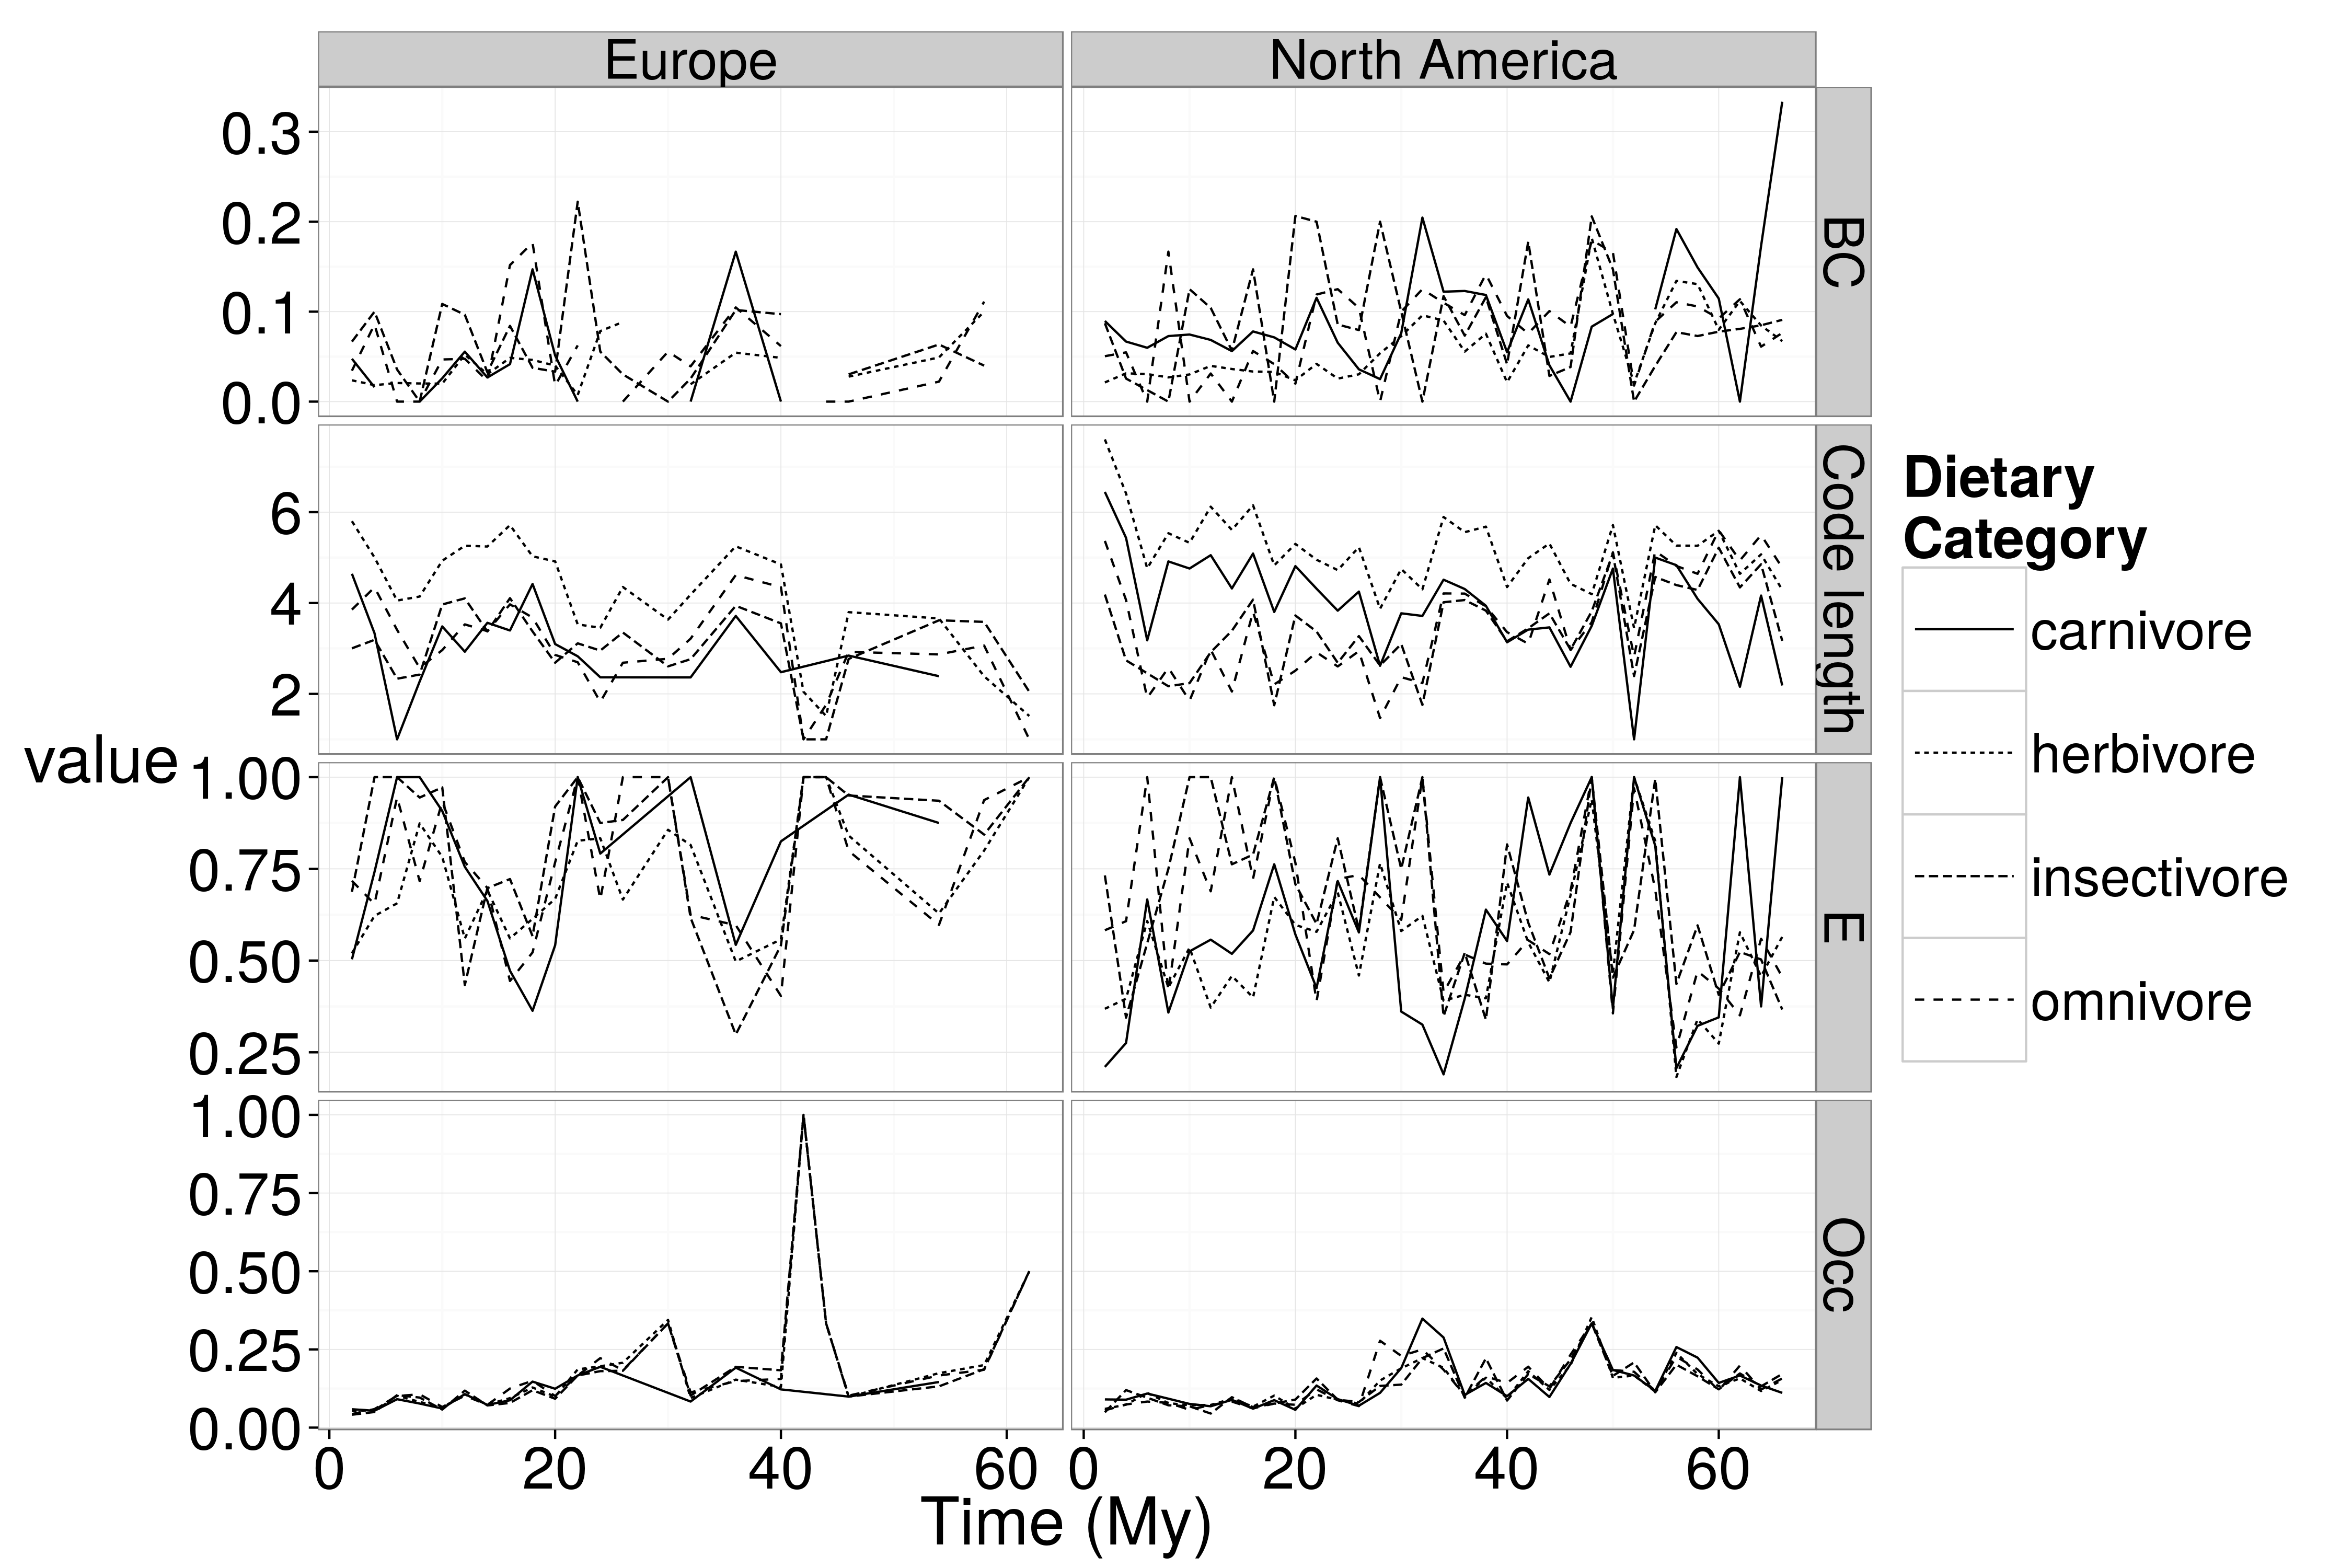
\includegraphics[width = \textwidth, height = 0.4\textheight, keepaspectratio = true]{figure/diets}
  \caption{Biogeographic network summary statistics for North American (right) and European (left) species-level occurrence information. From top to bottom, these summaries are biogeographic connectedness (BC), code length, relative number of taxa unique to a locality (E), and the relative taxon provincial occupancy (Occ). Measures are separated based on dietary category. Missing values are due to poor sampling in that bin.}
  \label{fig:com}
\end{figure}

Preliminary results show that mammal biome similarity is generally volatile through out the Cenozoic (Fig. \ref{fig:com}). Relative taxon provincial occupancy is relatively constant for most of the Cenozoic with a few spikes during periods of poor spatial sampling. Code length, a measure of the number and uniqeness of biomes, shows increasing separation between dietary categories during the Cenozoic. Both biogeographic connectedness and the relative number of taxa unique to a locality fluctuate the most though it appears to be mostly random movement around a constant mean.

Future analysis of these network measures will be done as a hierarchical Bayesian time series model where, for each continent, the different ecological combinations are exchangeable samples from a common underlying continent-specific mammalian distributional pattern. Because only two continents are currently sampled, stable estimates of an additional hierarchical level where continents are drawn from a common underlying global mammal distributional pattern is not possible \citep{Gelman2013d}. The inclusion of a third continent, South America, would allow for potentially stable estimates of a underlying common global mammal distributional pattern. %This is discussed further below.

\subsection{Extinction risk}
How ecology affects extinction risk is extremely important for having a more mechanistic understanding of the differential proliferation of taxa. Related to this is the Law of Constant Extinction which states that extinction is taxon age independent \citep{VanValen1973}. I use the mammalian fossil record to measure both the effect of ecology on taxon duration as well as taxon age upon extinction. 

Species durations will be modeled in a survival analysis framework where the effect of the above traits can be quantified as the effect upon a taxon's duration. This approach has a long history in paleobiology \citep{Simpson1944,Simpson1953,VanValen1973,VanValen1979,Baumiller1993,Foote1988} that has matured greatly as this analytical framework is commonly used in epidemiology, engineering, and demography studies \citep{Kleinbaum2005}. What makes survival analysis different from various linear modeling strategies such as logistic regression is that both duration and event occurrence are incorporated explicitly. In logistic regression, for example, only event occurrence is modeled, while in linear regression only duration is modeled. Importantly, because some taxa may have originated before the Cenozoic or not have gone extinct yet, this information can be explicitly modeled as a censored duration which increases the total information included in the model. 

Many paleontological analyses of extinction selectivity and survivorship are performed at the generic level \citep{Tomiya2013,Liow2008,Harnik2013,Finnegan2008,Foote2006} though there are potential biases in accurately modeling a specific level process using generic level data \citep{Raup1975,Sepkoski1975,Simpson2006,Raup1991a,VanValen1979}. Differences in species and generic level extinction risk can be attributed to speciation. Namely, if a trait has no effect on extinction risk at the specific level but decreases generic extinction risk this difference is most likely caused by differences in speciation rate. Because of this potentially elucidating property, I will be analyzing both species and generic level extinction risk. Importantly, this moves beyond simple analysis of diversification rates by partially decomposing the two aspects of diversification: speciation and extinction.

The current analyses are restricted to North America and Europe fossil occurrence information downloaded from both the PBDB and the NOW. Duration was measured as the difference between first appearance (FAD) and last appearance (LAD), in millions of years. This value is most certainly a truncated version of the true species duration and so some amount of correction must be made for sighting failure \citep{Alroy2014a,Solow1997,Strauss1989}. As with the study of community connectedness described above, dietary and locomotor assignments for each species were taken from the PBDB and the NOW. Body size estimates are based on a combination of measurement data from the PBDB, NOW, and a species by species literature search. These estimates are based on the common practice of using regression equations for estimating mass from measures such as tooth area or skull length \citep{Alroy1998,Tomiya2013,Jernvall2004,Alroy2009,Slater2013a}. 

Preliminary analyses were performed solely within a maximum likelihood and multi-model inference framework. Duration information was fit to either an exponential or Weibull distribution which are both common distributions for waiting times. The exponential distribution is a special case of the Weibull distribution where the scale (acceleration-deceleration) parameter \(k\) is set to 1. This means that the exponential distribution corresponds to age-independent extinction or the Law of Constant Extinction \citep{VanValen1973} while the Wiebull distribution allows for age-dependence. Dietary and locomotor categories were broken up into \(r - 1\) binary predictor variables, where \(r\) is the number of unique states for both traits, for a total of five binary predictors. A constant term was also estimated which corresponds to the remaining dietary and locomotor states. For North America the final biological predictor was natural log of body mass. Body size has not yet been included in the analysis of the European record that data collection effort is not yet been completed. As is common practice, the \(k\) parameter of the Weibull distribution was estimated as a single constant \citep{Kleinbaum2005}.

%\begin{wrapfigure}{r}{0.5\textwidth}
\begin{figure}[ht]
  \centering
  \begin{subfigure}[b]{0.48\textwidth}
    \caption{}
    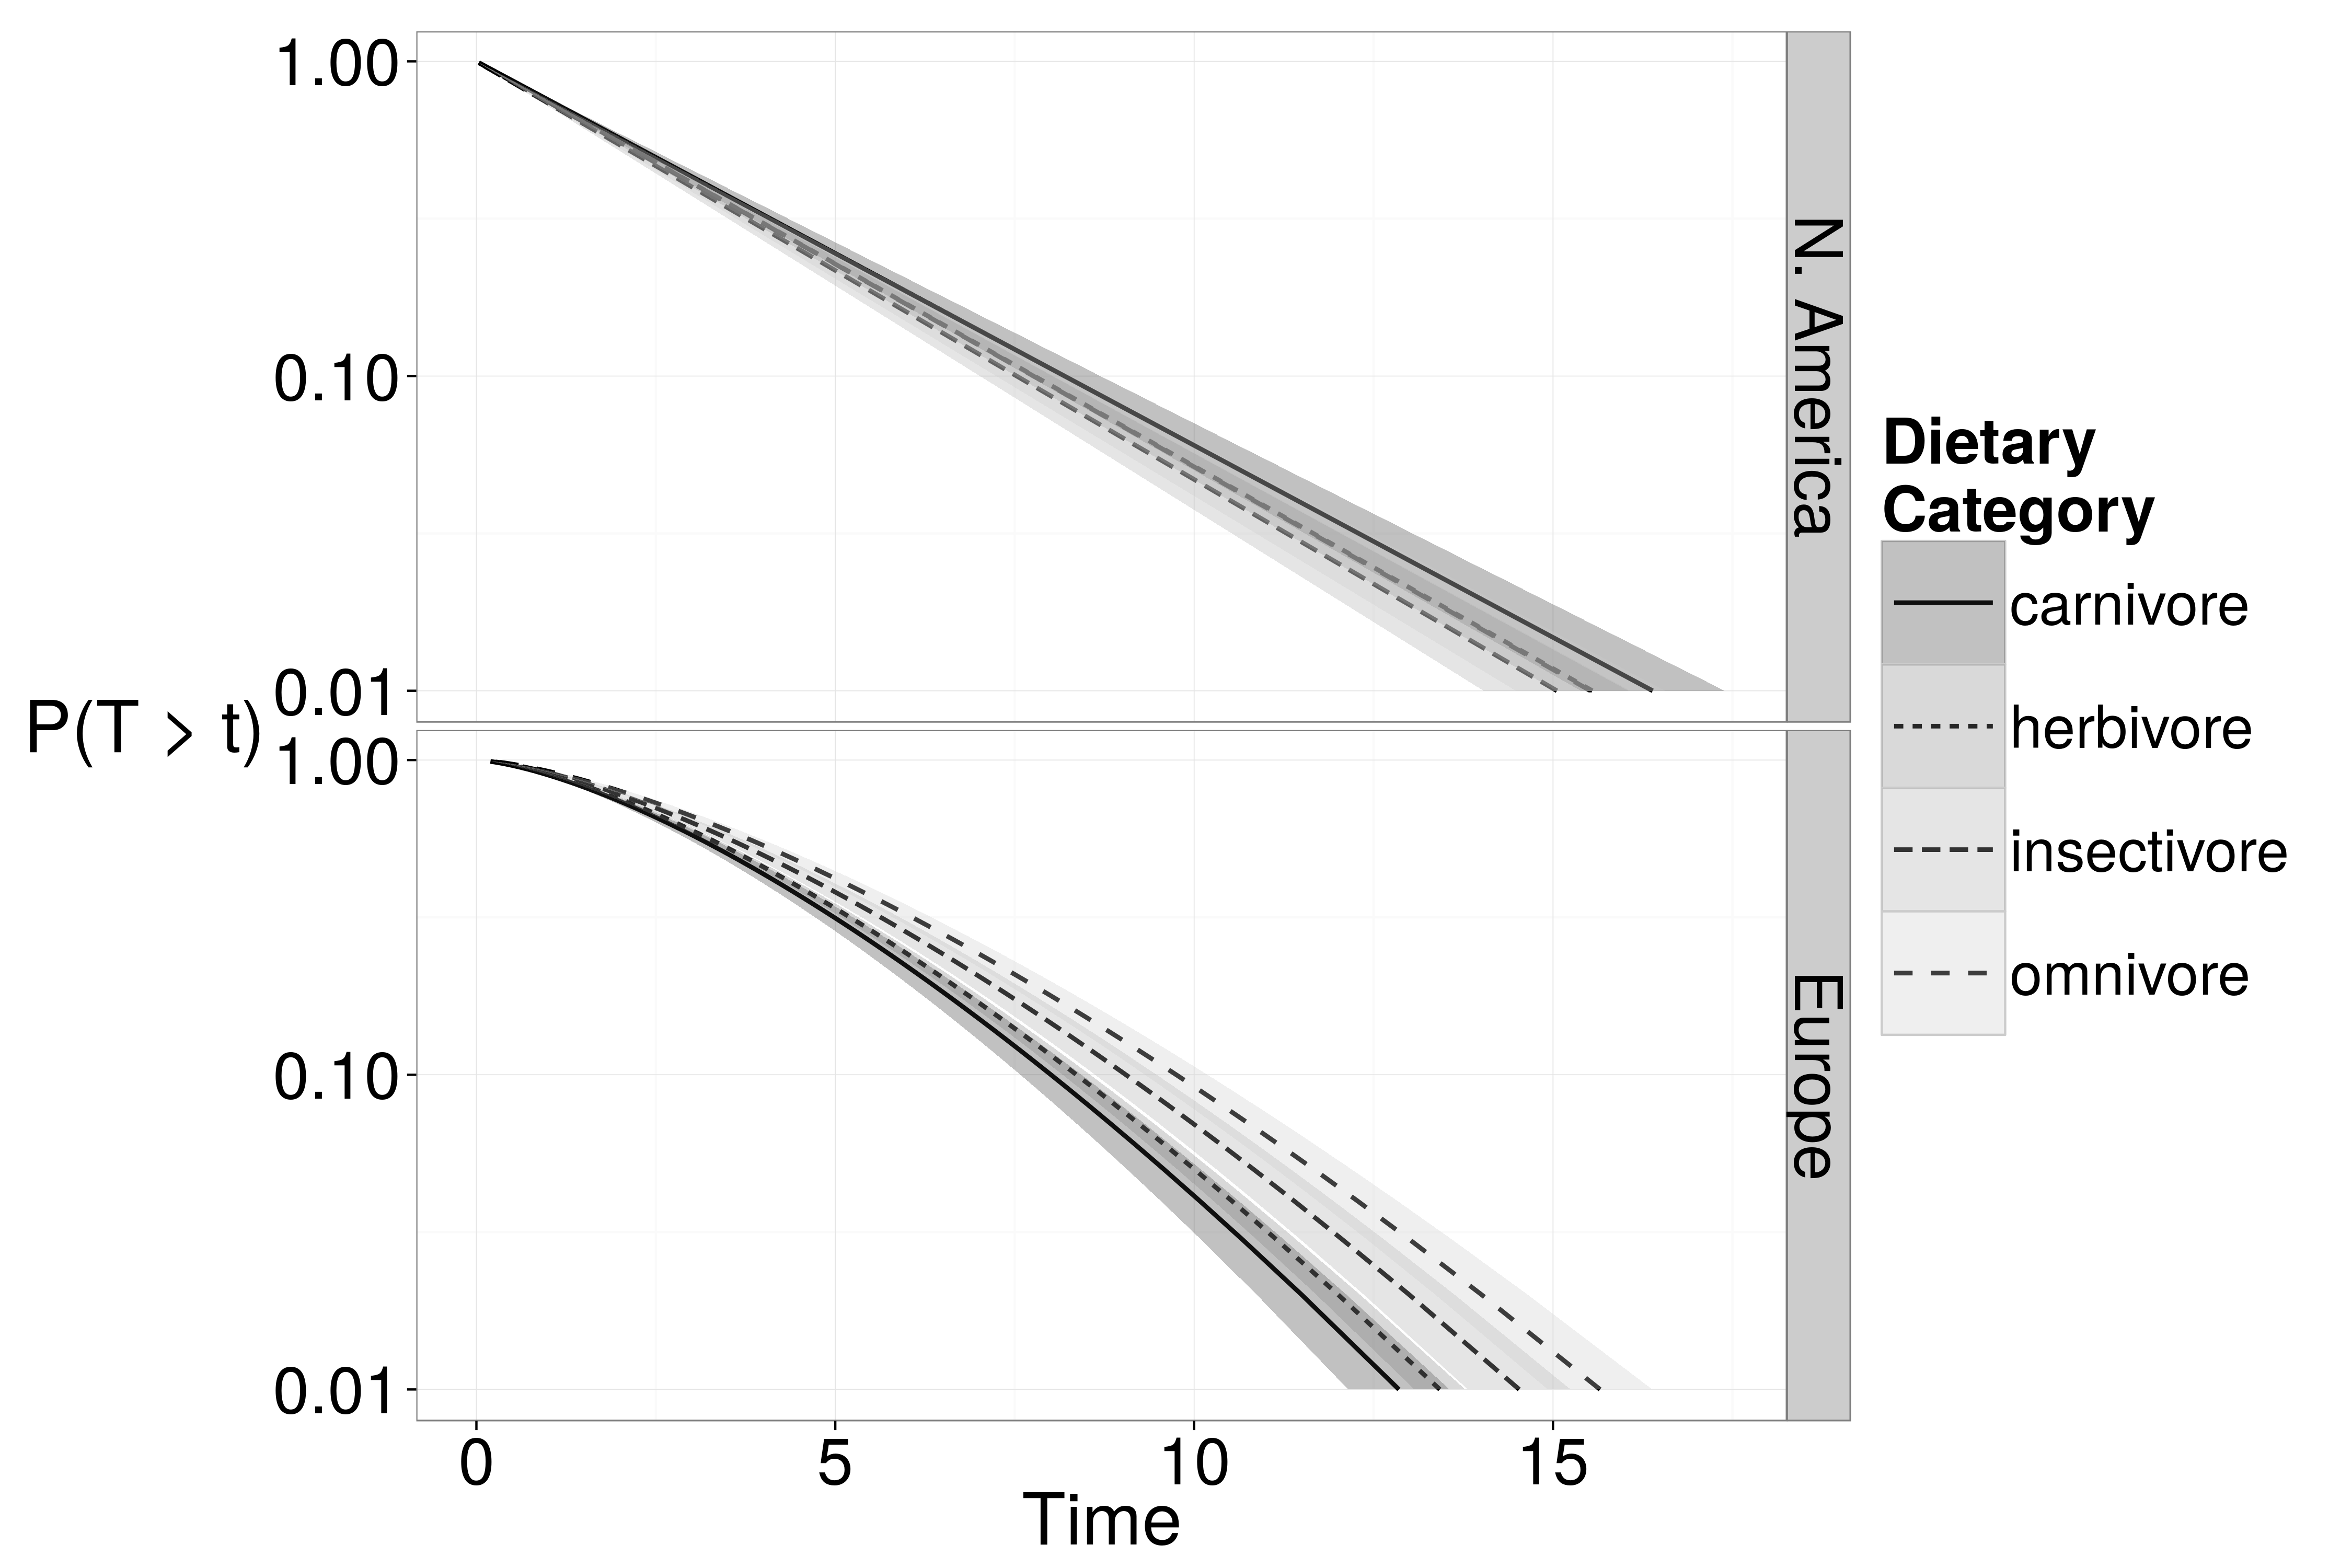
\includegraphics[width = \textwidth, keepaspectratio = true]{figure/para_diet}
    \label{subfig:diet}
  \end{subfigure}
  \begin{subfigure}[b]{0.48\textwidth}
    \caption{}
    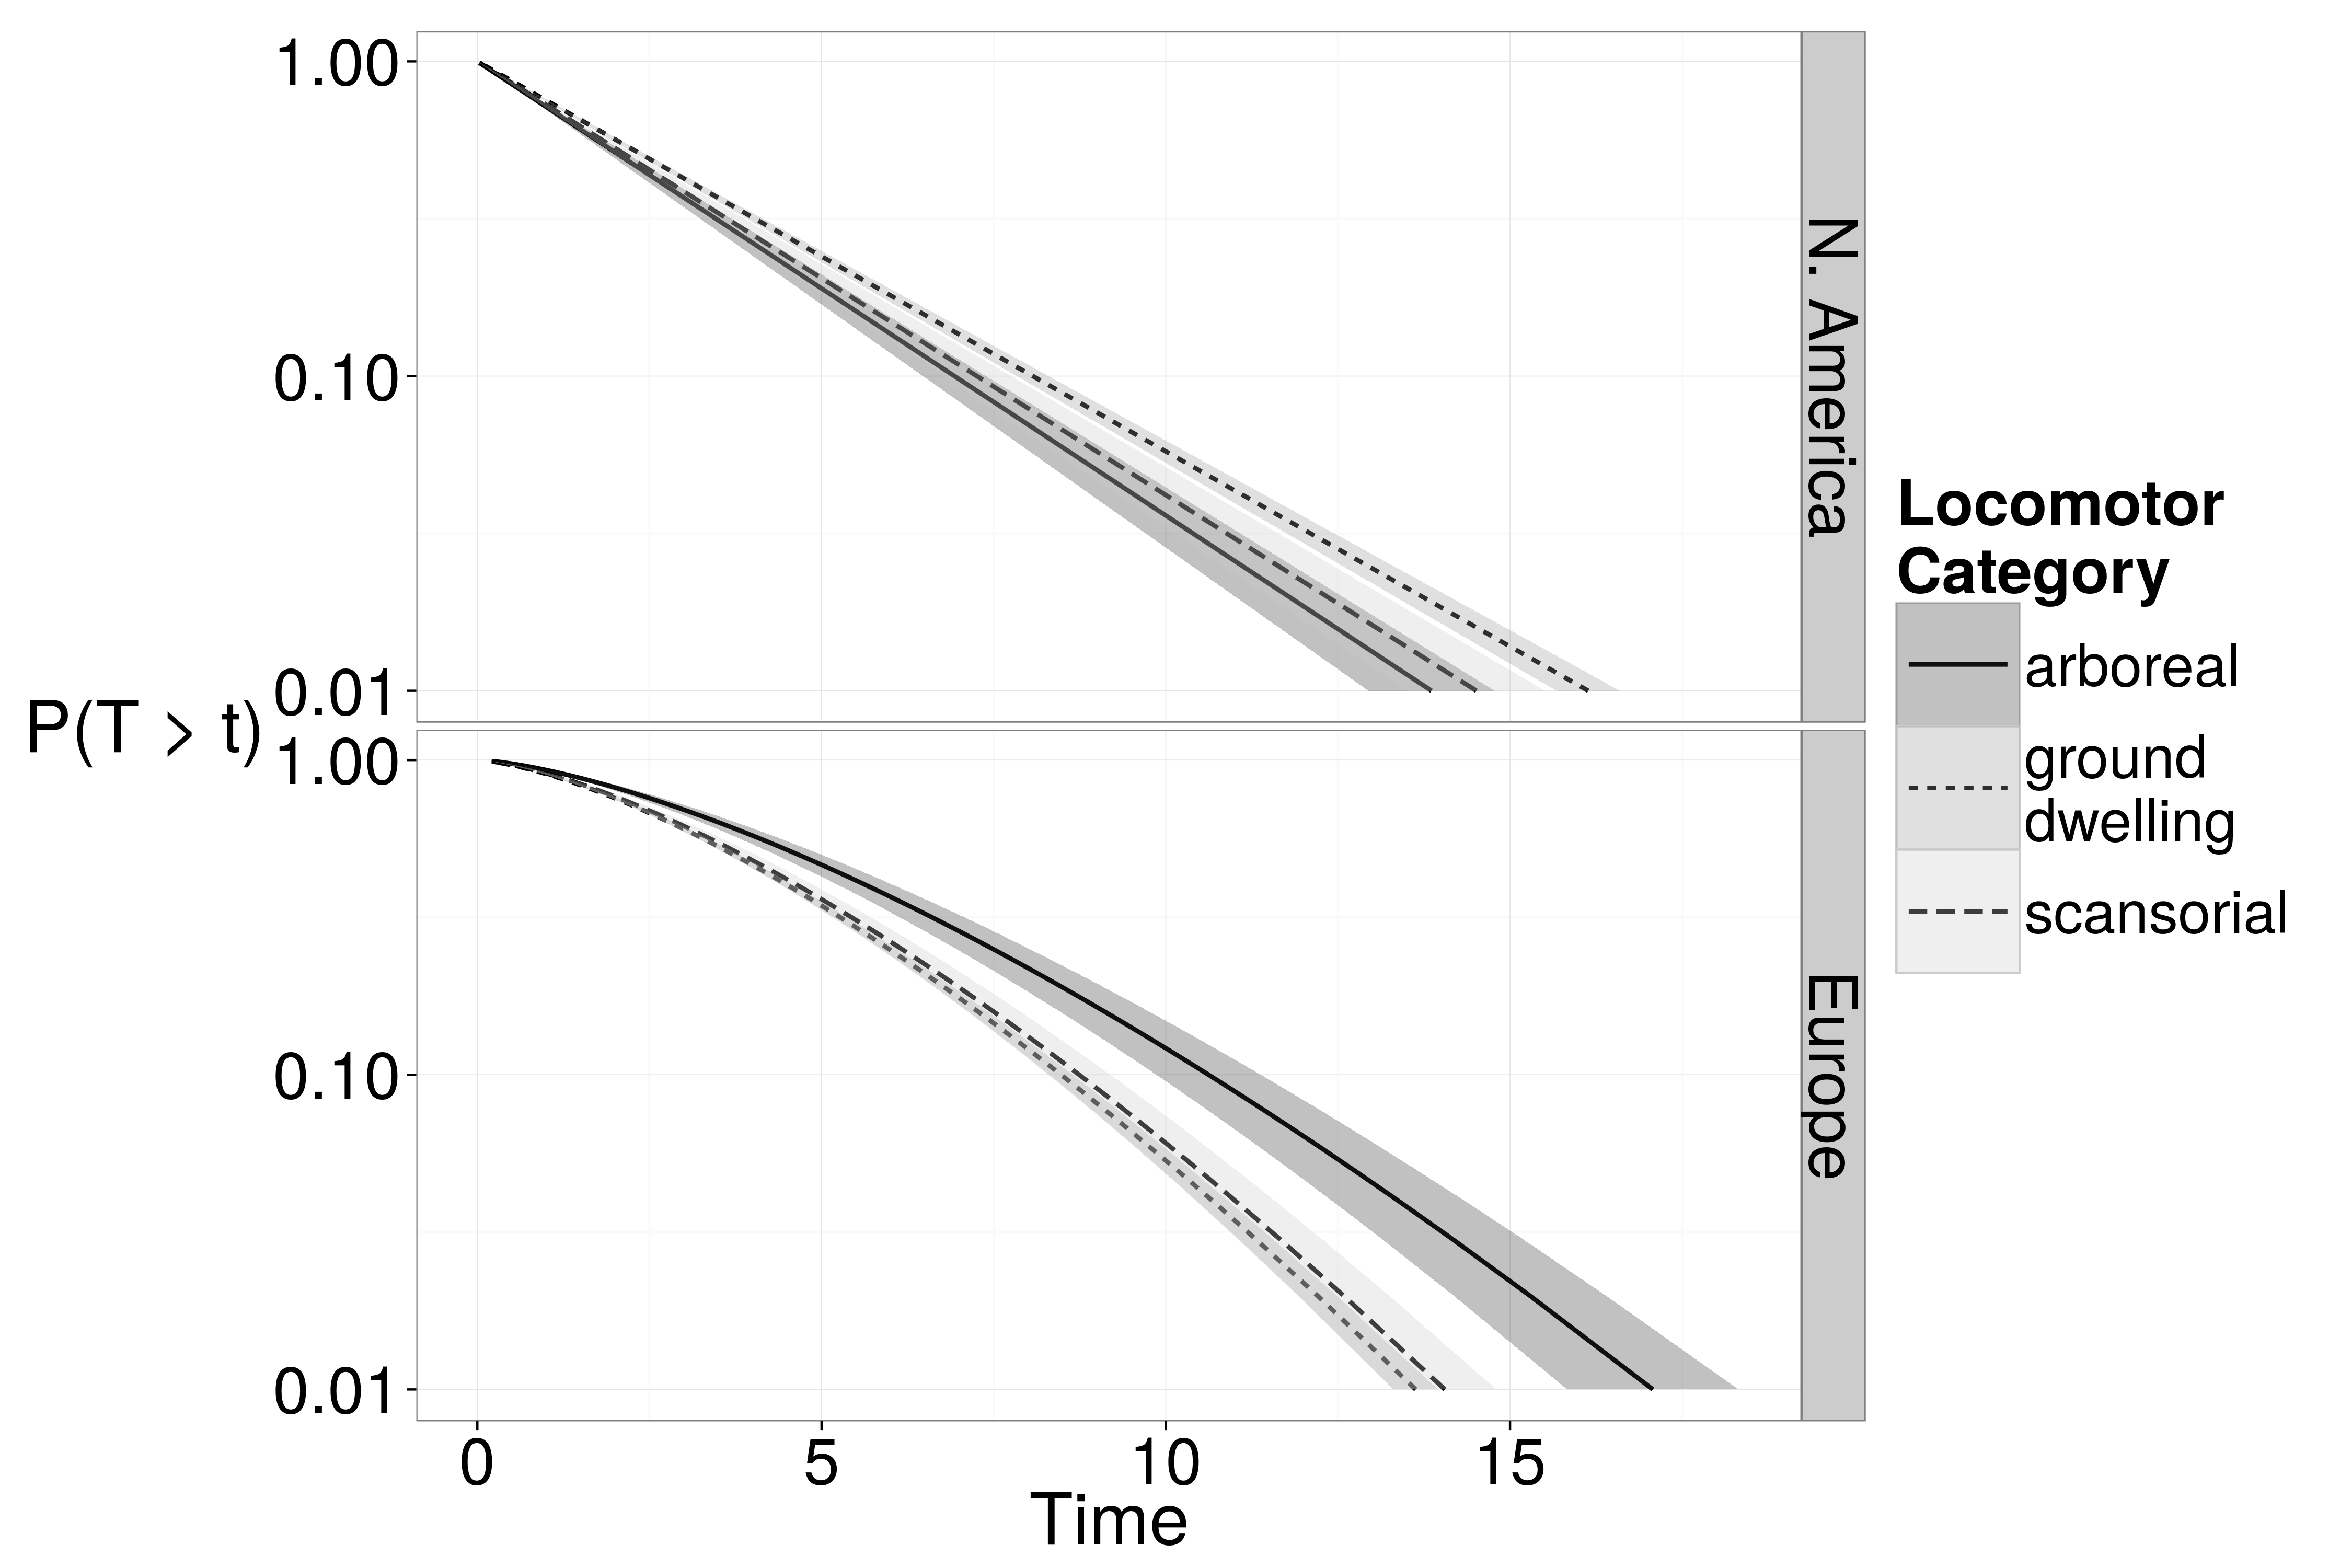
\includegraphics[width = \textwidth, keepaspectratio = true]{figure/para_move}
    \label{subfig:loco}
  \end{subfigure}
  \caption{Survival curves for mammal species based on dietary (\subref{subfig:diet}) and locomotor category (\subref{subfig:loco}) for North America and Europe. North American curves are from an exponential model while European survival curves are from a Weibull model. Distribution choice is based on model selection results. This curve is an estimate that a species will survive till time \(T\) having survived until time \(t\).}
  \label{fig:surv}
%\end{wrapfigure}
\end{figure}

Because of the volume of preliminary results, presented here are survival functions based on dietary and locomotor category for both North American and European species (Fig.~\ref{fig:surv}). There are pronounced differences between the survival patterns of these two continents. North American species show little variation in extinction risk based on diet with carnivore taxa being on average the longest lived while in Europe the differences are more striking with omnivorous taxa followed by insectivorous being the longest lived on average (Fig.~\ref{subfig:diet}). For both North America and Europe, locomotor category appears to have more effect upon extinction risk with North American ground dwelling taxa and European arboreal taxa being the longest lived on average for their respective continents (Fig.~\ref{subfig:loco}).

In future analyses, measures of climate and geographic range wll also included as continuous predictors of duration. Climate will be proxied via mean \(\delta O^{18}\) isotope value as calculated from \citet{Zachos2008} over the duration of the species. Mean provincial occupancy over the duration of the species will be calculated using the network theoretic approach described above.

Future modeling work will be done in a purely Bayesian framework in order to 1) better quantify the uncertainty with which estimates are made, 2) combine the analysis of the different continents in a hierarchical framework in order to estimate a common underlying distribution of survival times, 3) incorporate phylogenetic distance into a prior on a frailty coefficient \citep{Banerjee2003a,Ibrahim2001} to account for potential phylogenetic autocorrelation in species durations, and 4) to move on a continuous model expansion framework as opposed to a discrete model choice one \citep{Gelman2013d}. All of these changes will dramatically improve the interpretability and meaning of the results. Importantly, estimates under goal 2 would not be possible without the inclusion the inclusion of a third continent, South America. 

A unique aspect of the South American record is the presence of multiple ungulate-like orders that are rare or absent from other continents (e.g. Notoungulata) \citep{Marshall1982,Macfadden1997,Macfadden2006,Flynn1998a}. These convergent orders combined with the other ungulate-like orders present in North American and Europe make it possible to estimate, in a hierarchical Bayesian framework, the order specific distributions of taxon durations as well as the underlying distribution common to all ungulate-like taxa \citep{Gelman2013d}.


\section{Broader impacts}

My past and current research are based out of natural history museum collections which has let me be involved in some wonderful outreach programs. In Seattle, I participated for my entire undergraduate experience as an expert on both marsupial mammals and fossil mammals with the ``Meet the Mammals'' and ``Dino Day'' programs at the Burke Museum of Natural History and Culture. These programs were designed specifically to reach out to children and provide them the opportunity to see and touch specimens, providing the opportunity to interact directly with the museums collections. I plan to continue to participate in similar outreach programs at the Field Museum of Natural History in Chicago in order to possibly inspire future scientists. % need to be specific. Email Ken and Rick.

Most of the literature on South American fossil mammals is in Spanish and is effectively unavailable to many researchers. One of my goals with this study is to open up this literature. Related to this, I plan to learn conversational Spanish so that I can engage with students and other researchers in South America about my project. I am committed to providing whatever data I gather will be made available through the Dryad data archiving service (\url{http://datadryad.org/}) and will be entered into the Paleobiological Database (PBDB, \url{http://paleodb.org/} so that South America will continue to be included in future paleobiological studies. 

Mental health of students and researchers is both important and an ingetest of mine. My time spent on campuses around the world has let me observe many of the different and complex scenarios people encounter and have to over come. I (PDS) recently became involved with GSMHAB, a graduate student group involved with outreach, communication, and improvement of mental health services on the University of Chicago campus. The group specifically targets graduate students which make up two-thirds of the campus' student population. Additionally, I will be serving as a peer mentor to entering first-year graduate students through the SAIL program at the university.



\bibliography{proposal}

\end{document}
